% Условная компиляция для самостоятельной работы
\ifdefined\mainfile
    % Если это часть основного файла, не добавляем начало и конец документа
\else
    \documentclass[12pt, a4paper]{report}
    \usepackage{/Users/vladbelousov/Desktop/Semestr_4-FP-NSU/Настройка/library}
    \usepackage[utf8]{inputenc} % Подключение поддержки UTF-8
    \begin{document}
\fi

%%-------------------------------%%


\section{Материальные уравнения в Фурье-представлении}

\[ \frac{d \vec{p } }{dt } = - k \vec{r }_e (t )+ e \vec{r }_e (t )  \] 

\( \frac{d \vec{ r } _e }{dt }= \frac{\vec{ p } }{\gamma m }   \Rightarrow \text{ в }  \vec{r } _e (t ) \)   в следствие инерции электрона аккумулируется история (память) о воздействии.

Электрическим полем в предыдущие моменты времени \( t' \)  ,  а \( \vec{r } _e        \) дает вклад в \( \vec{P } (r,t) \). В общем случае линейная связь \( \vec{D }     \)  и \( \vec{E}  \)  полей имеет вид: 

\[ \vec{D } (\vec{r } ,t )= \vec{E } (\vec{r } , t )+ 4 \pi \vec{P } (\vec{r } , t ) = \frac{1}{(2 \pi ) ^2 } \iiiint \varepsilon(\vec{r } , \vec{r '} , t ,t ' ) \vec{E } (\vec{ r' } ,t' ) d ^3 r ' dt ' \quad ( t '< t ) \] 

Зависимость \( \varepsilon  \)  от \( \vec{r ' }  \)  возникает в случае переноса в веществе заряженных частиц (или обладающих дипольным моментом) из других точек среды.

Упрощения: 

1) Если среда стационарная и ее свойства зависят только от \( \vec{E }       \)  и \( \vec{ H}  \) и ни от ничего другого, то \( \varepsilon ( \vec{r } ,\vec{r '} , t,t ' ) =\varepsilon ( \vec{r } ,\vec{r ' } ,t -t ')  \) 

2) Если среда однородная \( \varepsilon ( \vec{r } ,\vec{r ' } ,t ,t' ) =\varepsilon ( \vec{r } - \vec{r' } , t ,t') \) 

Если среда однородная и стационарная, то 

\[ \vec{D } ( \vec{r } ,t )= \frac{1}{(2 \pi ) ^2 } \iiiint \varepsilon ( \vec{r }- \vec{r '} , t - t' ) \vec{E }  ( \vec{r' } ,t ') d ^3 r ' d t' \text{ (свертка)}    \] 

Используем преобразование Фурье на \( \vec{D}  \) :

\[ \hat{\vec{D } }(\vec{k } ,\omega )=  \hat{\varepsilon}( \vec{k } , \omega ) \hat{\vec{E }}   ( \vec{k}, \omega ); \quad \hat{\vec{B} } ( \vec{k } , \omega ) = \hat{\mu } ( \vec{k } , \omega) \hat{\vec{H }}  (\vec{k }  , \omega) \] 

% Сами в уравнение Максвелла подставите 

\( \displaystyle \frac{\omega ^2 }{c ^2 }\hat{\varepsilon}  (\vec{k } , \omega )\hat{\mu} ( \vec{k } , \omega)= k ^2 \)    - дисперсионное уравнение \( \to       \)   связь \( \omega   \) и \( \vec{k }  \) в среде.

Далее рассматриваем только твердое тело \( \Rightarrow  \varepsilon  \) и \( \mu     \)  зависят только от \( \omega \) 

\[ \frac{\omega ^2 }{c ^2 } \varepsilon( \omega ) \mu ( \omega) = k ^2   \] 

\( \underset{\text{без док-ва} }{\text{Для плазмы } } \)  \( \displaystyle \varepsilon ( \omega ) \simeq 1- \frac{\omega _p ^2 }{\omega ^2 } , \text{ } \omega _ p ^2 = \frac{4 \pi n_p e ^2 }{m } , \text{ } \mu ( \varepsilon ) = 1    \) 

\[ \frac{\omega ^2 }{c ^2 } \left(  1 - \frac{\omega _p ^2}{\omega ^2 }  \right) =k ^2 \Rightarrow \omega ^2 = \omega_p ^2  + k ^2 c ^2   \] 

\begin{center}
    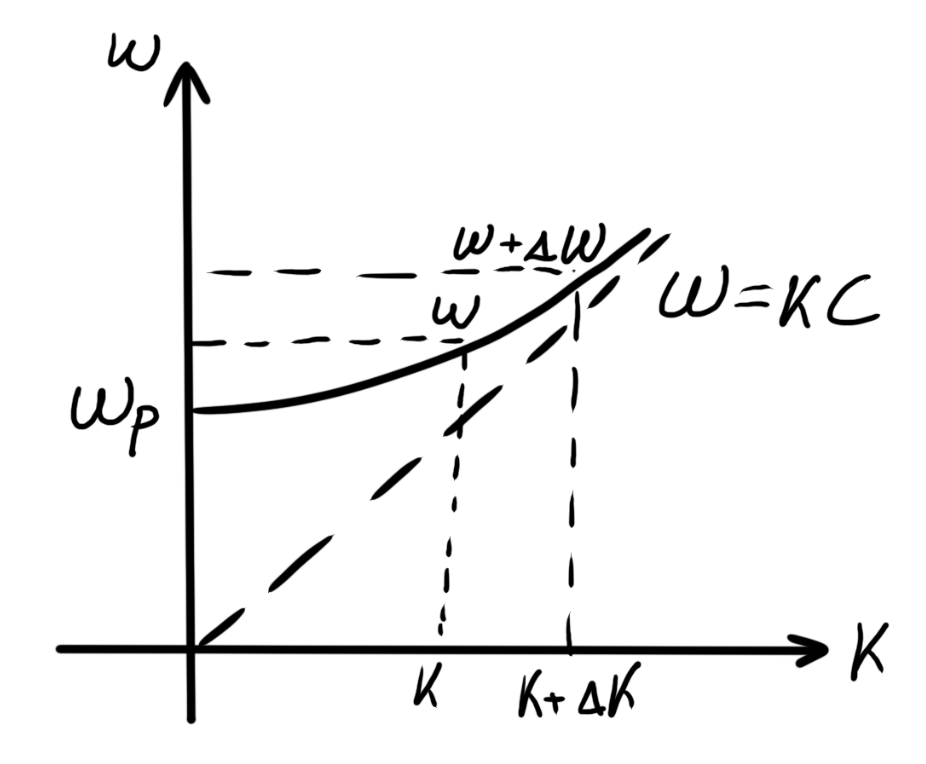
\includegraphics[width=0.4\textwidth]{/Users/vladbelousov/Desktop/Semestr_4-FP-NSU/ЭиО/Лекции_по_дням/image/26.png}
\end{center}

\section{Частотная дисперсия показателя преломления сред. Фазовая групповая скорость}

\[ \vec{E } (z,t ) = \vec{E_0 }e^{ikz - i \omega t }  , \text{ где } \frac{\omega ^2 }{c ^2 }\varepsilon ( \omega )\mu( \omega ) =k ^2    \] 

\( e^{ikz - i \omega t }=e^{ik(z- \frac{\omega}{k } t  )} ;   \) фаза волны \( kz - \omega t = \varphi( z, t ) \) 

\[ \varphi ( \vec{r } , t ) = ( \vec{k }  , \vec{r }  ) - \omega t  \] 

Если фаза \(\displaystyle  \varphi( z , t ) -  \) const, то  \( \displaystyle \frac{dz}{dt } = \frac{\omega}{k } = v_{\text{волны} } = \frac{c}{\sqrt{\varepsilon (\omega ) \mu ( \omega)}} =\frac{c}{ n ( \omega)}   \)

\( n ( \omega ) \) - показатель преломления среды. 

Ни энергия, ни информация не передается с \( v_{\Phi  }  \) (\( v_{\Phi  }  =v_{\text{волны} } \)), которая может быть больше \( c \) 

Рассмотрим монохроматическую волну, состоящую из двух монохроматических плоских волн, с близкой частотой: 

\[ \vec{E }  (z, t ) = \vec{E_0 }(\cos (kz - \omega t )+ \cos  ( (k+ \Delta k)z - ( \omega +\Delta \omega )t))=\]

\[ = \vec{E_0 } 2 \cos \left( \left( k+ \frac{\Delta k}{2}  \right)z - \left( \omega + \frac{\Delta \omega}{2}  \right) \right) \cos \left(  \frac{\Delta k }{2} z - \frac{\Delta \omega }{2 }  t   \right), \quad t=\text{const }     \] 

\begin{center}
    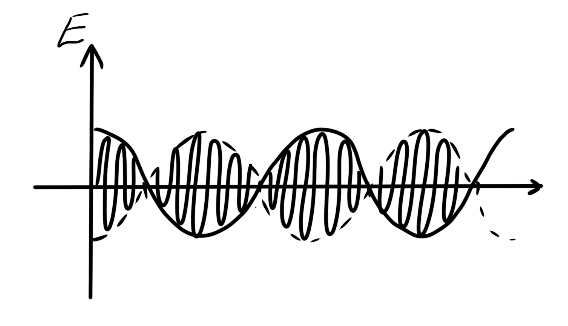
\includegraphics[width=0.5\textwidth]{/Users/vladbelousov/Desktop/Semestr_4-FP-NSU/ЭиО/Лекции_по_дням/image/27.png}
\end{center}

Скорость движения огибающей: 

\[ \frac{\Delta k z }{ 2 }  - \frac{\Delta \omega t }{2 }  = \mathrm{const }  \Rightarrow \frac{dz}{dt } = \frac{ \Delta \omega }{\Delta k } = \boxed {\frac{d \omega }{ dk }  = v_{g}} - \text{ групповая скорость}     \] 

Соотношения Рэлея \( \displaystyle \frac{\omega n( \omega)}{c }  = k \text{ (дисперсионное уравнение)} \Rightarrow   \) 

\[ \frac{d}{d \omega} ( \omega n ( \omega)) = \frac{ dk c }{d \omega } \] 

\[  n(\omega ) + \omega \frac{dn( \omega )}{d \omega } = \frac{dk}{d \omega } c \Rightarrow   \frac{d \omega } {dk } = \frac{ c }{ n( \omega ) + \omega \frac{ dn (\omega)}{d \omega} }  =       \] 

\[ =\underbrace{ \frac{c}{ n ( \omega )}}_{v_{\Phi } } \frac{1}{ 1+ \frac{\omega}{n ( \omega )}\frac{dn}{d \omega}  }  \Rightarrow v_g = \frac{v_{\Phi} } {1+ \frac{\omega}{ n } \frac{dn}{d \omega}  }   \] 

Если \( \displaystyle  \frac{dn}{d \omega }> 0   \) , то \( v_g< v_{\Phi}  \) - нормальная дисперсия

Если  \( \displaystyle  \frac{dn}{d \omega }< 0   \) , то \( v_g>v_{\Phi}  \) - аномальная дисперсия

\section{Движение одномерного волнового пакета в среде с дисперсией \( \omega = \omega( k ) \) }

Известно, что он движется по \( z \) 

\begin{center}
    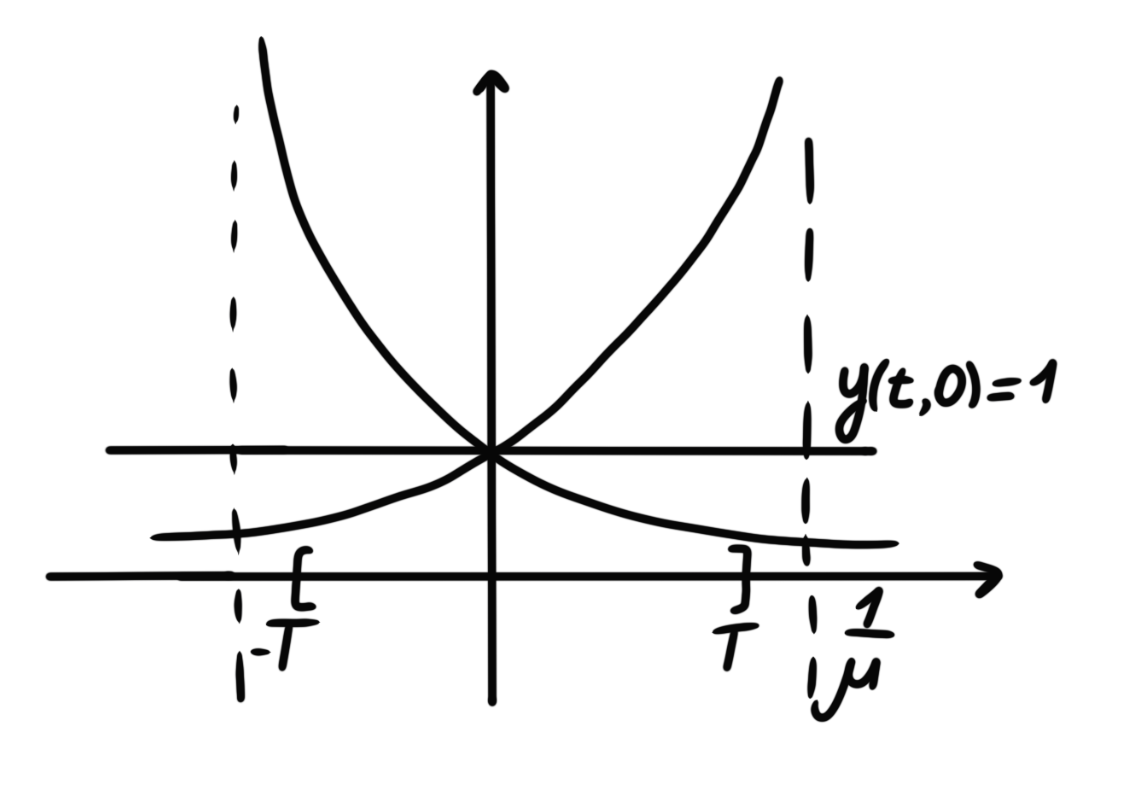
\includegraphics[width=0.5\textwidth]{/Users/vladbelousov/Desktop/Semestr_4-FP-NSU/ЭиО/Лекции_по_дням/image/28.png}
\end{center}

\[ \vec{E } ( z, 0 )= \vec{E_0 } ( z ) e^{i k_0 z}   \]

Используем преобразование Фурье на \( \vec{E}  \): 

\[ \hat{\vec{E }}   ( k ) =\frac{1}{\sqrt{2 \pi } } \int_{-\infty}^{\infty} \underbrace{\vec{E_0}  (z ) e^{i k_0 z }}_{=\vec{E }  (z,0)} e^{- ik z } dz =\hat{ \vec{E_0}  }( k- k_0 )      \] 

Для электрического поля волны с \( k  \)  эволюция во времени описывается: 

\[ \vec{E }  ( k ) e^{ikz - i\omega(k ) t }  \] 

\[ \vec{E }  ( z, k  ) =\frac{1}{\sqrt{2 \pi}}  \int_{-\infty}^{\infty} \vec{E }  ( k ) e^{ikz - i\omega(k ) t }   dk\] 

\begin{center}
    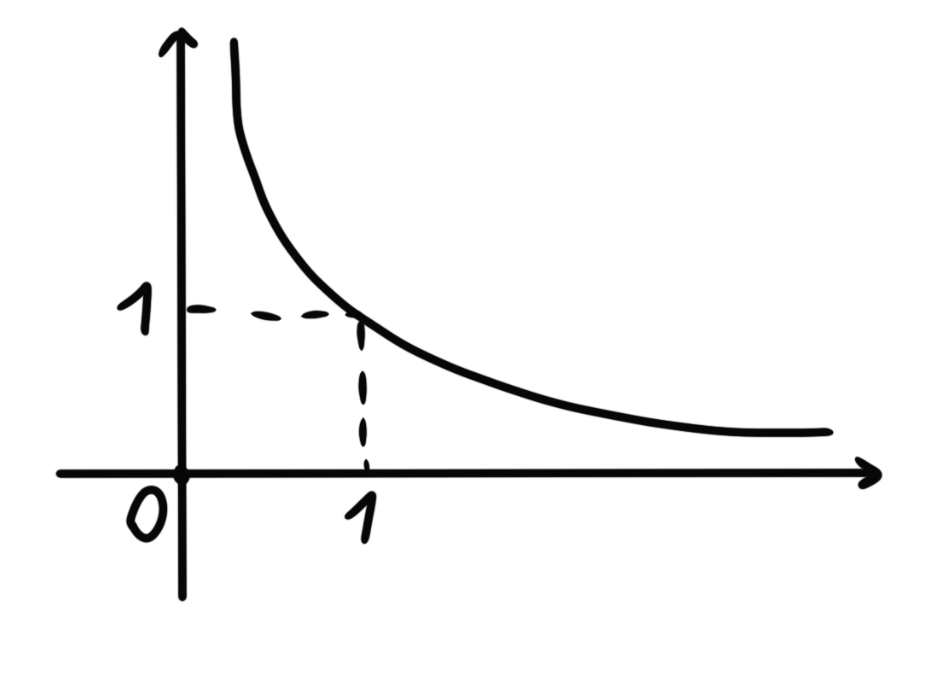
\includegraphics[width=0.5\textwidth]{/Users/vladbelousov/Desktop/Semestr_4-FP-NSU/ЭиО/Лекции_по_дням/image/29.png}
\end{center}

Если \(\displaystyle  \lambda = \frac{2\pi}{k_0} \ll   \) масштаб изменения \( E_0(z ) \) или длины пакета \( L_0 \)  

\begin{center}
    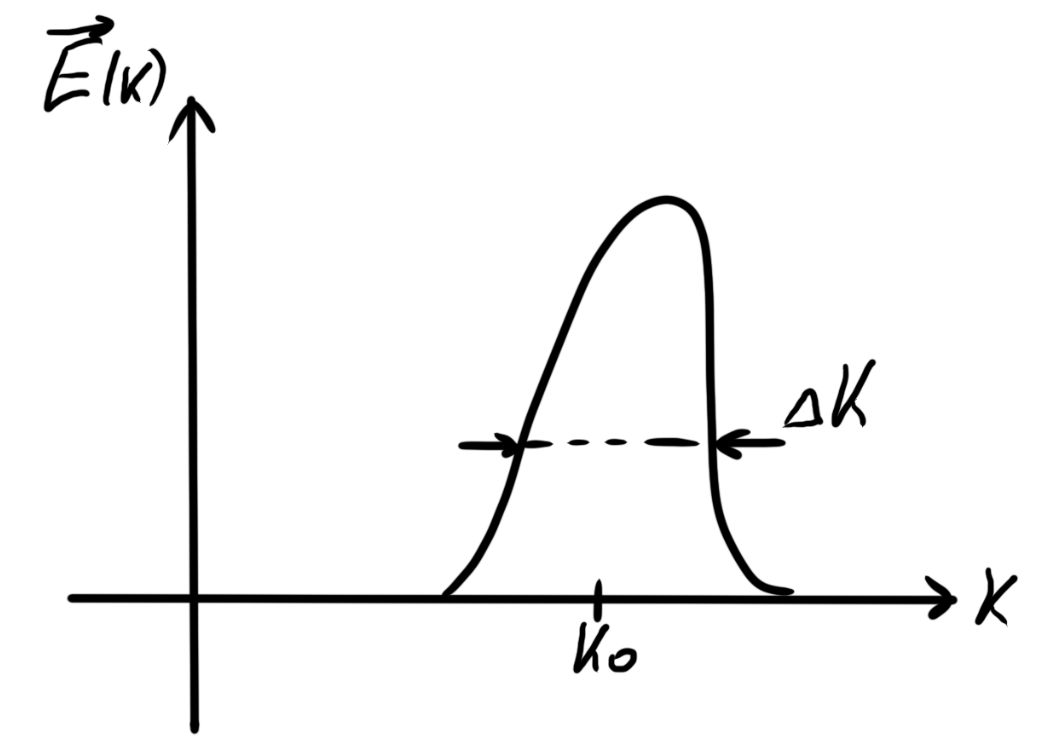
\includegraphics[width=0.5\textwidth]{/Users/vladbelousov/Desktop/Semestr_4-FP-NSU/ЭиО/Лекции_по_дням/image/30.png}
\end{center}

\[ \Delta k L_0 \sim \pi \Rightarrow \Delta k \sim \frac{\pi}{L_0}   \] 

\[ k \sim k_0 \sim \frac{2 \pi }{\lambda} \Rightarrow \frac{\Delta  k }{k_0 } \ll 1     \] 

%рис

\[ \omega ( k ) \simeq \underbrace{\omega( k_0 )}_{\omega_0} + \frac{d \omega }{ dk} \bigg|_{k_0}  (k- k_0 ) + \cancelto{0_{\text{т.к мал} } }{\frac{1}{ 2 }  \frac{ d ^2 \omega } { d k ^2 }  \bigg|_{k_0}  (k-k_0 ) ^2}     \] 

1) Пусть \(\displaystyle  \omega ( k ) = \omega_0 + v_g ( k-k_0 ) ; \vec{E } ( z,t ) = \frac{1}{\sqrt{2 \pi } } \int_{-\infty}^{\infty}  \vec{E }  ( k ) e^{ikz - \omega_0t - i v_gt ( k-k_0)}  dk = \) 

\[ \frac{ e^{i k_0 v_gt -i \omega t} }{\sqrt{2\pi } }\int_{-\infty}^{\infty}  E(k ) e ^{i k (z- v_gt )}dk  = e^{i k_0 v_gt - i \omega_0 t} \vec{E_0} ( z- v_gt ) e^{i k_0 (z- v_gt )}= \vec{E_0} ( z- v_gt  ) e^{i k_0 z - i \omega_0 t }        \] 

- пакет без изменения формы движется по z 

2) Учтем \( \displaystyle i\frac{d ^2\omega }{dk ^2 } \bigg |_{k = k_0}  \frac{(k-k_0 ) ^2 }{2} \Delta t  \ll i \frac{\pi}{2 }  \Rightarrow \Delta t = \frac{\pi}{\Delta k ^2 \omega ''}\sim \frac{ L_0 ^2 }{ \pi \omega ''}        \) 

Если \( \displaystyle t \gg \Delta t    \quad  \frac{\Delta v_g }{\Delta k } \sim \frac{d v_g }{dk } = \frac{d \left( \frac{d \omega}{dk}  \right)}{dk}= \omega '' (k_0 ) \Rightarrow \Delta v_g \simeq \omega '' (k_0 )\Delta k       \) 

Расплывания пакета: \( \Delta L= \Delta v_g t \simeq \omega '' ( k_0 ) \Delta k t   \) 

\[ L(t  ) \simeq \sqrt{L_0 ^2 + \Delta L  ^2 } = \sqrt{ L_0 ^2 + ( \omega '' (k_0  )\Delta k t) ^2 }   \] 

Примеры дисперсионных соотношений: 

1) Электромагнитна волна, в вакууме, звук в среде \( \omega = k a , \text{ }  a = \mathrm{const}   \) 

\begin{center}
    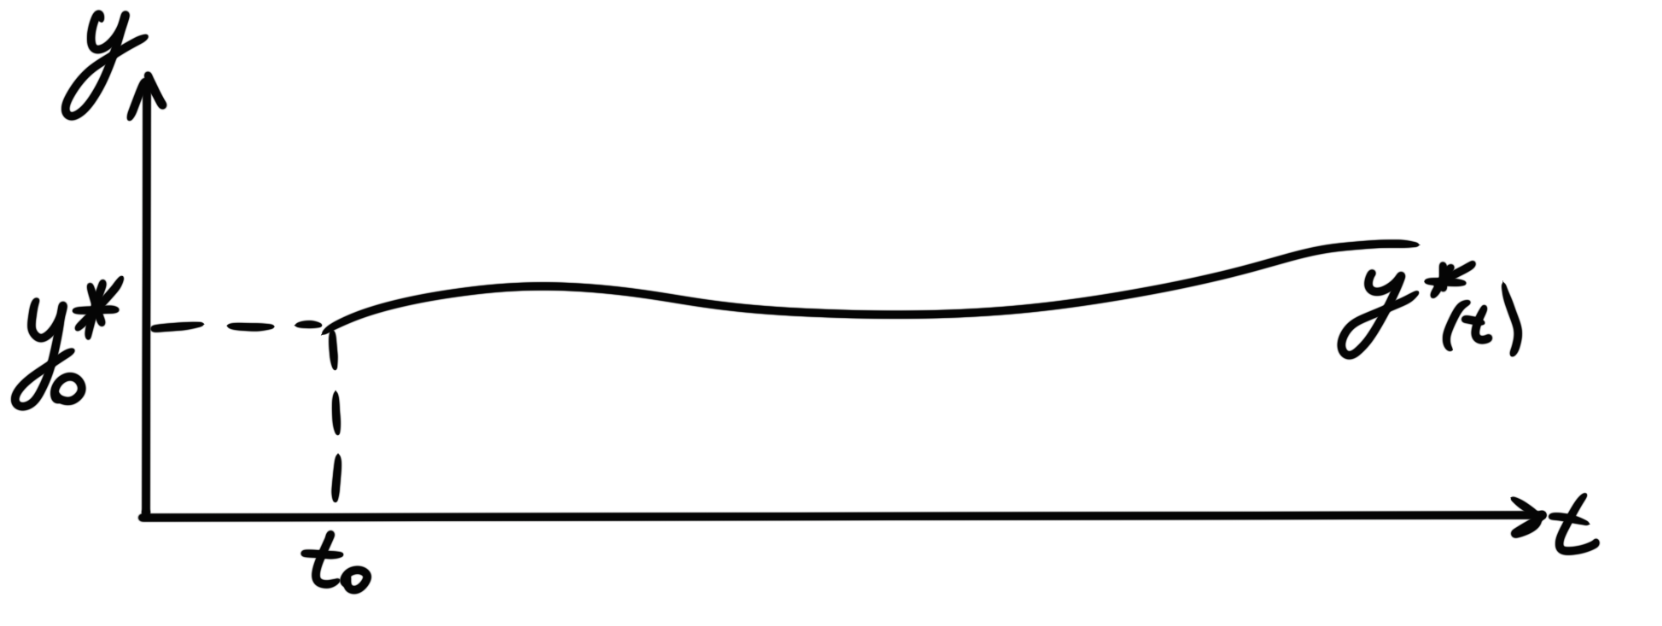
\includegraphics[width=0.3\textwidth]{/Users/vladbelousov/Desktop/Semestr_4-FP-NSU/ЭиО/Лекции_по_дням/image/31.png}
\end{center}

\[ v_{\Phi  } = \frac{\omega}{ k }  = a, \text{ }  v_g = \frac{ d \omega }{ d k}= a    \] 

2) \( \omega = \sqrt{gk } \) - волны на поверхности жидкости: 

\begin{center}
    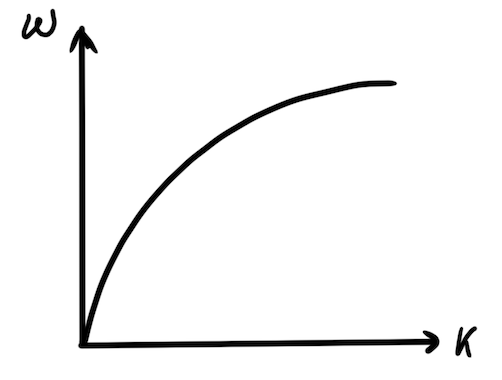
\includegraphics[width=0.3\textwidth]{/Users/vladbelousov/Desktop/Semestr_4-FP-NSU/ЭиО/Лекции_по_дням/image/32.png}
\end{center}

\[ v_{\Phi } = \sqrt{\frac{g}{k} }, \text{ }  v_g = \frac{1}{ 2} \sqrt{\frac{g}{k} } \Rightarrow v_g< v_{\Phi}     \] 

3) Электромагнитная волна в плазме: \( \omega ^2 = \omega_p ^2 + k ^2 c ^2  \) 

\begin{center}
    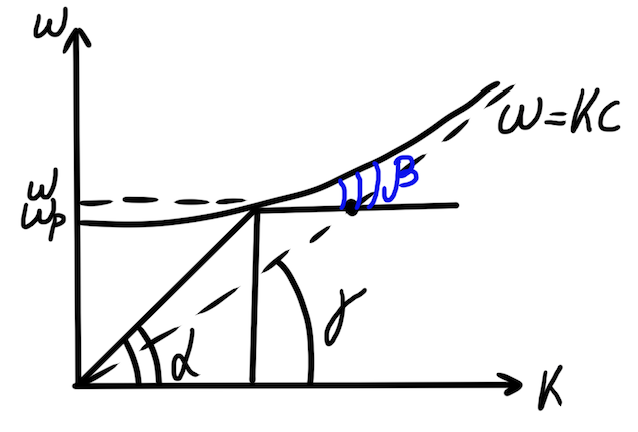
\includegraphics[width=0.3\textwidth]{/Users/vladbelousov/Desktop/Semestr_4-FP-NSU/ЭиО/Лекции_по_дням/image/33.png}
\end{center}

\[ v_{\Phi }  = \frac{\sqrt{ \omega_p ^2 + k ^2  c ^2 }}{k }, \text{ }  v_g = \frac{d \omega }{dk } =\frac{1}{2 }  \frac{2 k c ^2 }{\sqrt{ \omega_p + k ^2 c ^2 }} = \frac{ c ^2 }{v_{\Phi} } , v_g v_{\Phi }  = c ^2   \] 

\[ v_{\Phi } = tg \alpha, \text{ }  v_g = \frac{d \omega } {dk } = tg \beta , \text{ }  tg \gamma = \frac{\omega}{k }  = c   \] 

\[ \alpha > \gamma , \text{ }  \beta < \gamma \Rightarrow \alpha  > \beta - \text{ нормальная дисперсия}  :  \] 

\[ tg \alpha > tg \beta ,\quad v_{\Phi }> v_g  \] 





%%-------------------------------%%

% Закрытие документа, если файл компилируется отдельно
\ifdefined\mainfile
    % Если это основной файл, не нужно заканчивать документ
\else
    \end{document}
\fi